\documentclass[a4paper,12pt]{article} % добавить leqno в [] для нумерации слева
\usepackage[a4paper,top=1.3cm,bottom=2cm,left=1.5cm,right=1.5cm,marginparwidth=0.75cm]{geometry}
%%% Работа с русским языком
\usepackage{cmap}					% поиск в PDF
\usepackage{mathtext} 				% русские буквы в фомулах
\usepackage[T2A]{fontenc}			% кодировка
\usepackage[utf8]{inputenc}			% кодировка исходного текста
\usepackage[english,russian]{babel}	% локализация и переносы

\usepackage{graphicx}

\usepackage{wrapfig}
\usepackage{tabularx}

\usepackage{hyperref}
\usepackage[rgb]{xcolor}
\hypersetup{
colorlinks=true,urlcolor=blue
}
\usepackage{multirow}
\usepackage{hhline}


%%% Дополнительная работа с математикой
\usepackage{amsmath,amsfonts,amssymb,amsthm,mathtools} % AMS
\usepackage{icomma} % "Умная" запятая: $0,2$ --- число, $0, 2$ --- перечисление

%% Номера формул
\mathtoolsset{showonlyrefs=true} % Показывать номера только у тех формул, на которые есть \eqref{} в тексте.

%% Шрифты
\usepackage{euscript}	 % Шрифт Евклид
\usepackage{mathrsfs} % Красивый матшрифт

%% Свои команды
\DeclareMathOperator{\sgn}{\mathop{sgn}}

%% Перенос знаков в формулах (по Львовскому)
\newcommand*{\hm}[1]{#1\nobreak\discretionary{}
{\hbox{$\mathsurround=0pt #1$}}{}}

\begin{document}
	
	\begin{titlepage}
	\begin{center}
		{\large МОСКОВСКИЙ ФИЗИКО-ТЕХНИЧЕСКИЙ ИНСТИТУТ (НАЦИОНАЛЬНЫЙ ИССЛЕДОВАТЕЛЬСКИЙ УНИВЕРСИТЕТ)}
	\end{center}
	\begin{center}
		{\large Физтех-школа электроники, фотоники и молекулярной физики}
	\end{center}
	
	
	\vspace{4.5cm}
	{\huge
		\begin{center}
			{Лабораторная работа 2.1.1}\\
			Измерение удельной теплоемкости воздуха при постоянном давлении
		\end{center}
	}
	\vspace{2cm}
	\begin{flushright}
		{\LARGE Салтыкова Дарья \\
			\vspace{0.5cm}
			Б04-105}
	\end{flushright}
	\vspace{8cm}
	\begin{center}
		Долгопрудный 2022
	\end{center}
\end{titlepage}

\section{Введение}

\textbf{Цель работы:} 1) измерить повышение температуры воздуха в зависимости от мощности подводимого тепла и расхода при стационарном течении через трубу; 
2) исключив тепловые потери, по результатам измерений определить теплоёмкость воздуха при постоянном давлении.
\medskip

\noindent \textbf{Оборудование:} теплоизолированная стеклянная трубка; электронагреватель; источник питания постоянного тока; амперметр; вольтметр (цифровые мультиметры); термопара, подключённая к микровольтметру; компрессор; газовый счётчик; секундомер.

\section{Теоретические сведения}

\noindent Измерение теплоёмкости тел обычно производится в калориметрах, т.е. в сосудах, обеспечивающих теплоизоляцию исследуемого тела от внешней среды. При этом регистрируется изменение его температуры $\delta T$ в зависимости от количества тепла $\delta Q$, полученного телом от некоторого нагревательного элемента внутри калориметра. Теплоёмкость тела в некотором процессе определяется как их отношение:


\begin{equation}
\begin{aligned}
C = \dfrac{\delta Q}{\delta T} 
\end{aligned}
\end{equation}


\noindent Надёжность измерения определяется, в основном, качеством калориметра. Необходимо, чтобы количество тепла, затрачиваемое на нагревание исследуемого тела, существенно превосходило тепло, расходуемое на нагревание самого калориметра, а также на потери тепла из установки. При измерении теплоёмкости газов эти требования выполнить довольно трудно - масса газа в калориметре и, следовательно, количество тепла, идущее на его нагревание, как правило, малы. Для увеличения количества нагреваемого газа при неизменных размерах установки в нашей работе исследуемый газ (воздух) продувается через калориметр, внутри которого установлен нагреватель. При этом измеряются мощность нагревателя, масса воздуха, протекающего в единицу времени (расход), и приращение его температуры.

\begin{wrapfigure}{r}{0.6\textwidth}
  \begin{center}
    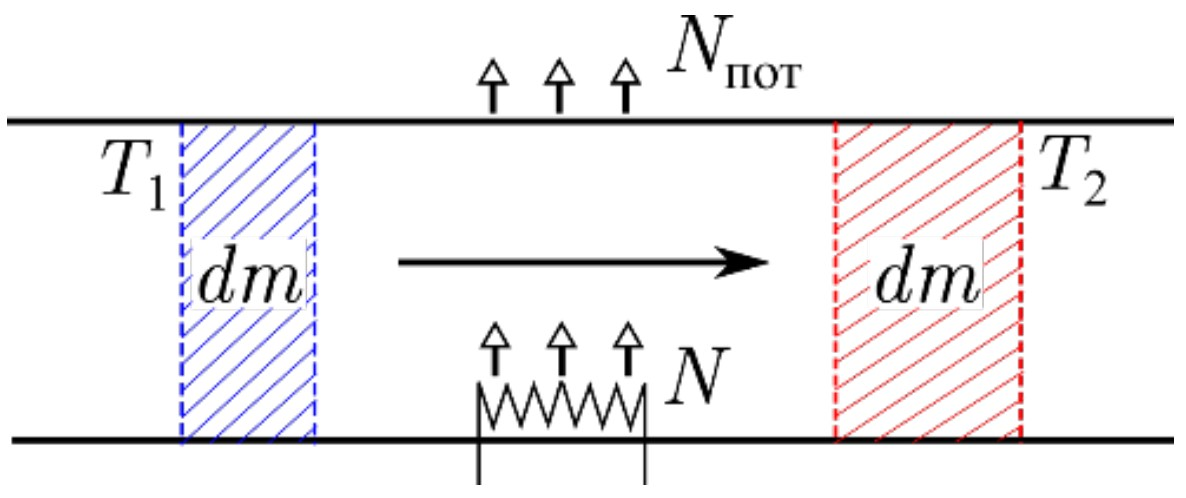
\includegraphics[width = 0.6\textwidth]{труба.JPG}
  \end{center}
  \caption{Нагрев газа при течении по трубе}
\end{wrapfigure}

\noindent Рассмотрим газ, протекающий стационарно слева направо через трубу постоянного сечения, в кото-рой установлен нагревательный элемент (см.рис.1). Пусть за некоторое время $dt$ через калориметр прошла малая порция газа массой $dm = q dt$ , где $q$ [кг/с] - массовый расход газа в трубе. Если мощность нагрева равна $N$, мощность тепловых потерь на обмен с окружающей средой $N_{\text{пот}}$, то порция получила тепло $\delta Q =(N - N_{\text{пот}})dt$. С другой стороны, по определению теплоёмкости
(1): $\delta Q =c dm \Delta T$ , где $\Delta T = T_2 - T_1$ - приращение температуры газа, и $c$ — удельная (на единицу массы) теплоёмкость газа в рассматриваемом процессе. При малых расходах газа и достаточно большом диаметре трубы перепад давления на её концах мал, поэтому можно принять, что $P_1 \approx P_2 = P_0$, где $P_0$ - атмосферное давление. Следовательно, в условиях опыта измеряется удельная теплоёмкость при постоянном давлении $c_P$. Таким образом, получаем

\begin{equation}
\begin{aligned}
C_p = \dfrac{N - N_{\text{пот}}}{q \Delta T} 
\end{aligned}
\end{equation}

\section{Экспериментальная установка}

\noindent Схема установки изображена на рис. 1. Воздух, нагнетаемый компрессором, прокачивается через калориметр. Калориметр представляет собой стеклянную цилиндрическую трубку с двойными стенками, запаянными с торцов. На внутреннюю поверхность стенок трубки нанесено серебряное покрытие для минимизации потерь тепла за счет излучения. Воздух из пространства между стенками калориметра откачан до высокого вакуума ($10^{-5}$ торр) для минимизации потерь тепла, обусловленных теплопроводностью.

\begin{center}
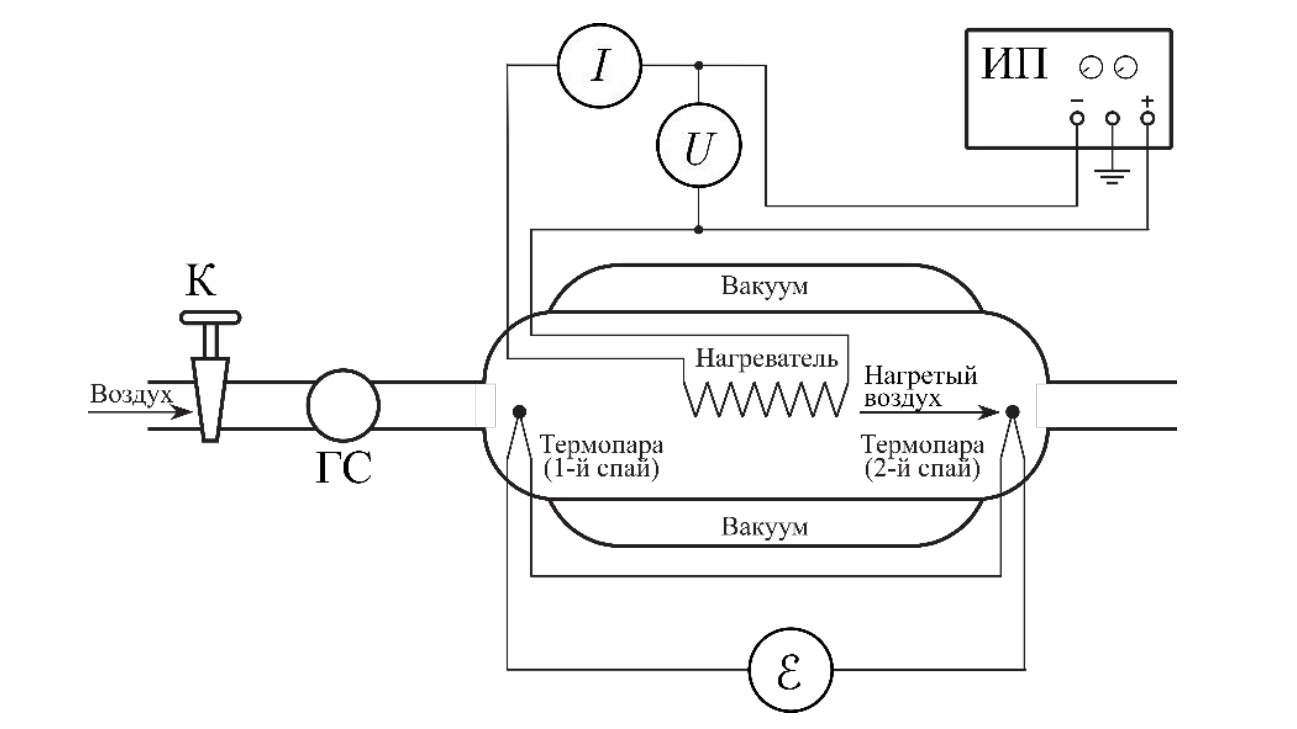
\includegraphics[width = 1\textwidth]{установка.jpg}
\end{center}

\noindent Нагреватель в виде намотанной на пенопласт нихромовой проволоки раcположен внутри калориметра непосредственно в воздушном потоке. Нагрев проволоки производится от регулируемого источника постоянного тока (ИП). Напряжение $U$ на нагревателе и ток $I$ через него регистрируются цифровыми мультиметрами. Таким образом, мощность нагрева равна

\begin{equation}
\begin{aligned}
N = UI 
\end{aligned}
\end{equation}

\noindent Для измерения разности температур $\Delta T$ служит медно-константановая термопара. Один спай термопары расположен в струе воздуха, входящего в калориметр, и находится при комнатной температуре, а второй - в струе выходящего нагретого воздуха. Константановая проволока термопары расположена внутри калориметра, а медные проводники подключены к цифровому вольтметру. Возникающая в термопаре ЭДС $\varepsilon$ пропорциональна разности температур $\Delta T$ спаев:

\begin{equation}
\begin{aligned}
\varepsilon = \beta \Delta T
\end{aligned}
\end{equation}

\noindent где $\beta = 40,7 \dfrac{\text{мкВ}}{ ^{\circ} C}$ - чувствительность медно-константановой термопары в рабочем диапазоне температур (20-30 $ ^{\circ} C$). ЭДС регистрируется с помощью микровольтметра.

\medskip

\noindent Объём воздуха, прошедшего через калориметр, измеряется газовым счётчиком ГС. Для регулировки расхода служит кран К. Время $\Delta t$ прохождения некоторого объема $\Delta V$ воздуха измеряется секундомером. Объёмный расход равен $\Delta V / \Delta t$, массовый расход может быть найден как

\begin{equation}
\begin{aligned}
q = \rho_0 \dfrac{\Delta V}{\Delta t} 
\end{aligned}
\end{equation}

\noindent где $\rho_0$ - плотность воздуха при комнатной температуре, которая в свою очередь может быть получена из уравнения Менделеева–Клапейрона: $\rho_0 = \dfrac{\mu P_0}{RT_0}$, где $P_0$ - атмосферное давление, $T_0$ - комнатная температура (в Кельвинах), $\mu$ = 29,0 г/моль - средняя молярная масса (сухого) воздуха.

\medskip

\noindent Учитывая особенности устройства калориметра, следует ожидать, что мощность нагревателя расходуется не только на нагрев массы прокачиваемого воздуха, но и частично теряется за счет нагрева внутренних стенок термостата и рассеяния тепла через торцы термостата. Можно предположить, что при небольшом нагреве ($\Delta T << T_0$) мощность потерь тепла $N_{\text{пот}}$ прямо пропорциональна разности температур:

\begin{equation}
\begin{aligned}
N_{\text{пот}} = \alpha \Delta T
\end{aligned}
\end{equation}

\noindent где $\alpha$ — некоторая константа. При этом условии основное соотношение (2) принимает вид

\begin{equation}
\begin{aligned}
N = (c_p q+ \alpha) \Delta T
\end{aligned}
\end{equation}

\noindent Следовательно, при фиксированном расходе воздуха ($q = const$) подводимая мощность и разность температур связаны прямой пропорциональностью ($\Delta T (N)$ — линейная функция).

\medskip

\section{Ход работы}

\medskip

\noindent 1. Подготовим к работе газовый счетчик: проверим, что он заполнен  водой, установим счетчик по уровню.

\medskip

\noindent 2. Охладим калориметр до комнатной температуры.

\medskip

\noindent 3. Включим вольтметр, предназначенный для измерения ЭДС термопары. 

\medskip

\noindent 4. Запишем показания компнатной температуры, давления и влажности. Вычислим плотность воздуха при данных условиях 

$$T_{0} = 23 \; ^\circ C, P_{0} = 99530 \text{ Па}, \varphi = 20\% $$

$$\rho = 1,17 \text{ кг/м3}$$

\noindent 5. С помощью газового счетчика и секундомера измерим максимальный расход воздуха $\frac{\Delta V}{\Delta T}$ (в л/с). Измерения представлены в таблице. 

\begin{table}[h!]
\begin{tabular}{|l|l|}
\hline
t, с  & dV/dt, л/с \\ \hline
24,7  & 0,202      \\ \hline
24,9  & 0,201      \\ \hline
24,81 & 0,202      \\ \hline
\end{tabular}
\end{table}

\noindent По найденным значениям определим среднее значение расхода и массовый расход воздуха $q_{max}$ [г/с].

$$\langle\frac{\Delta V}{\Delta t}\rangle = 0,202\text{ л/с}$$

$$q_{max} = 0,236\text{ г/с}$$

\noindent 6. Оценим величину тока нагревателя $I_{0}$, требуемого для нагрева воздуха на $\Delta T = 1\text{ К}$.

\medskip
 	
\noindent Оценим минимальную мощность $N_0$, необходимую для нагрева газа при максимальном расходе. $N_{0} = c_{p}q\Delta T \approx 0.238 \text{ Вт}.$
	
\medskip	
	
\noindent Учитывая, что сопротивление проволоки нагревателя составляет приблизительно $R \approx 35\text{ Ом}$ и в процессе опыта практически не меняется, искомое значение тока $I_{0} = q N_{0} R \approx 83 \text{ мА}.$
	
\medskip	
	
\noindent 7. Проведем измерение зависимости разности температур от мощности нагрева $\Delta T(N)$ при расходе воздуха $q = 0,236 \text{ г/с}.$ Погрешность измерения тока: $\sigma_{I} = 0.01 \text{ мA}$;  напряжения: $\sigma_{U}= 0.01 \text{ В}$, $\sigma_{\varepsilon}= 1 \text{ мВ}$.

\begin{table}[h!]
\begin{tabular}{|l|l|l|l|l|l|l|l|}
\hline
I, мА  & U, В  & $\varepsilon$, мкВ & R, Ом & N, Вт & $\sigma_N$,    Ом & $\Delta T$, К & $\sigma_T$, К \\ \hline
99,87  & 3,529 & 53,0            & 35,34 & 0,352 & 0,0010            & 1,30          & 0,00025       \\ \hline
114,67 & 4,051 & 71,0            & 35,33 & 0,465 & 0,0011            & 1,74          & 0,00025       \\ \hline
127,23 & 4,491 & 88,0            & 35,29 & 0,571 & 0,0013            & 2,16          & 0,00025       \\ \hline
147,91 & 5,218 & 119,0           & 35,27 & 0,767 & 0,0015            & 2,92          & 0,00025       \\ \hline
163,15 & 5,754 & 144,0           & 35,26 & 0,936 & 0,0016            & 3,54          & 0,00025       \\ \hline
179,97 & 6,346 & 176,0           & 35,26 & 1,141 & 0,0018            & 4,32          & 0,00025       \\ \hline
\end{tabular}
\end{table}
	
\noindent Завершив первую серию измерений, охладим калориметр до комнатной температуры.

\medskip

\noindent 8. Проведем аналогичные измерения для другого значения расхода воздуха.

\begin{table}[h!]
\begin{tabular}{|l|l|}
\hline
t, с  & dV/dt, л/с \\ \hline
18,38 & 0,1360     \\ \hline
18,59 & 0,1345     \\ \hline
18,43 & 0,1356     \\ \hline
\end{tabular}
\end{table}

$$\langle\frac{\Delta V}{\Delta t}\rangle = 0,135\text{ л/с}, q = 0,158 \text{ г/с}, N_0 = 0,157 \text{ Вт}, I_0 = 67 \text{ мА}$$

\begin{table}[h!]
\begin{tabular}{|l|l|l|l|l|l|l|l|}
\hline
I, мА  & U, В  & $\varepsilon$, мкВ & R, Ом & N, Вт & $\sigma_N$,    Ом & $\Delta T$, К & $\sigma_T$, К \\ \hline
86,54  & 3,054 & 54,0               & 35,29 & 0,264 & 0,0009            & 1,33          & 0,00025       \\ \hline
103,86 & 3,669 & 82,0               & 35,33 & 0,381 & 0,0010            & 2,01          & 0,00025       \\ \hline
120,14 & 4,246 & 112,0              & 35,34 & 0,510 & 0,0012            & 2,75          & 0,00025       \\ \hline
137,24 & 4,849 & 147,0              & 35,33 & 0,665 & 0,0014            & 3,61          & 0,00025       \\ \hline
153,15 & 5,408 & 184,0              & 35,31 & 0,828 & 0,0015            & 4,52          & 0,00025       \\ \hline
180,12 & 6,362 & 256,0              & 35,32 & 1,146 & 0,0018            & 6,29          & 0,00025       \\ \hline
\end{tabular}
\end{table}

\noindent После завершения опытов выключим источник питания нагревателя и мультиметры. Кран К откроем для максимального продува воздуха через калориметр.

\medskip

\noindent 9. Построим на одном графике зависимости $\Delta T (N)$ при разных значениях $q$ (Рис. 2).

\medskip

\noindent 10. Построим график зависимости $\frac{1}{k}(q)$ и, пользуясь формулой $N = (c_p q+ \alpha) \Delta T$, определим теплоёмкость воздуха при постоянном давлении $c_p$ (Рис. 3).

$$\frac{1}{k} = c_p q + \alpha$$

\begin{table}[h!]
\begin{tabular}{|l|l|l|l|l|}
\hline
k, Вт/К & $1/k$, К/Вт & $\sigma_{1/k}}$, К/Вт & q, г/с & $\sigma_q$, г/с \\ \hline
3,82    & 0,262               & 0,020                      & 0,236  & 0,002           \\ \hline
5,61    & 0,178               & 0,011                       & 0,158  & 0,001           \\ \hline
\end{tabular}
\end{table}

\noindent Получаем $$c_p = (1070 \pm 68)\frac{\text{Дж}}{\text{К кг}}$$

$$\alpha = (0,00906 \pm 0,0018) \frac{\text{Дж}}{\text{К с}}$$

\noindent 11. Вычислим доли тепловых потерь в опытах : $\frac{N_\text{пот}}{N} =\frac{\alpha}{k}$

\begin{table}[h!]
\begin{tabular}{|l|l|}
\hline
q, $\frac{\text{г}}{\text{с}}$ & Nпот/N   \\ \hline
0,236            & $(24 \pm 0,52)\cdot 10^{-4}
 $  \\ \hline
0,158            & $(16 \pm 0,47)\cdot 10^{-4}
$ \\ \hline
\end{tabular}
\end{table}


\section{Вывод}

\medskip 

\noindent В ходе работы было определено значение удельной теплоемкости воздуха при $T_{0} = 23 \; ^\circ C, P_{0} = 99530 \text{ Па}, \varphi = 20\% $: 

$$ (1070 \pm 68) \frac{ \text{Дж}}{\text{К кг}} $$

\noindent Табличное значение: $ c_{p_\text{табл}} = 1003 \frac{ \text{Дж}}{\text{К кг}}$

\medskip

\noindent В пределах погрешности значения совпадают.

\medskip

\noindent Также были определены доли тепловых потерь в опытах. В среднем $\frac{N_\text{пот}}{N} = (20 \pm 0,50) \cdot 10^{-4}.$


\section{Графики}	

\begin{figure}[h!]
	\begin{center}
		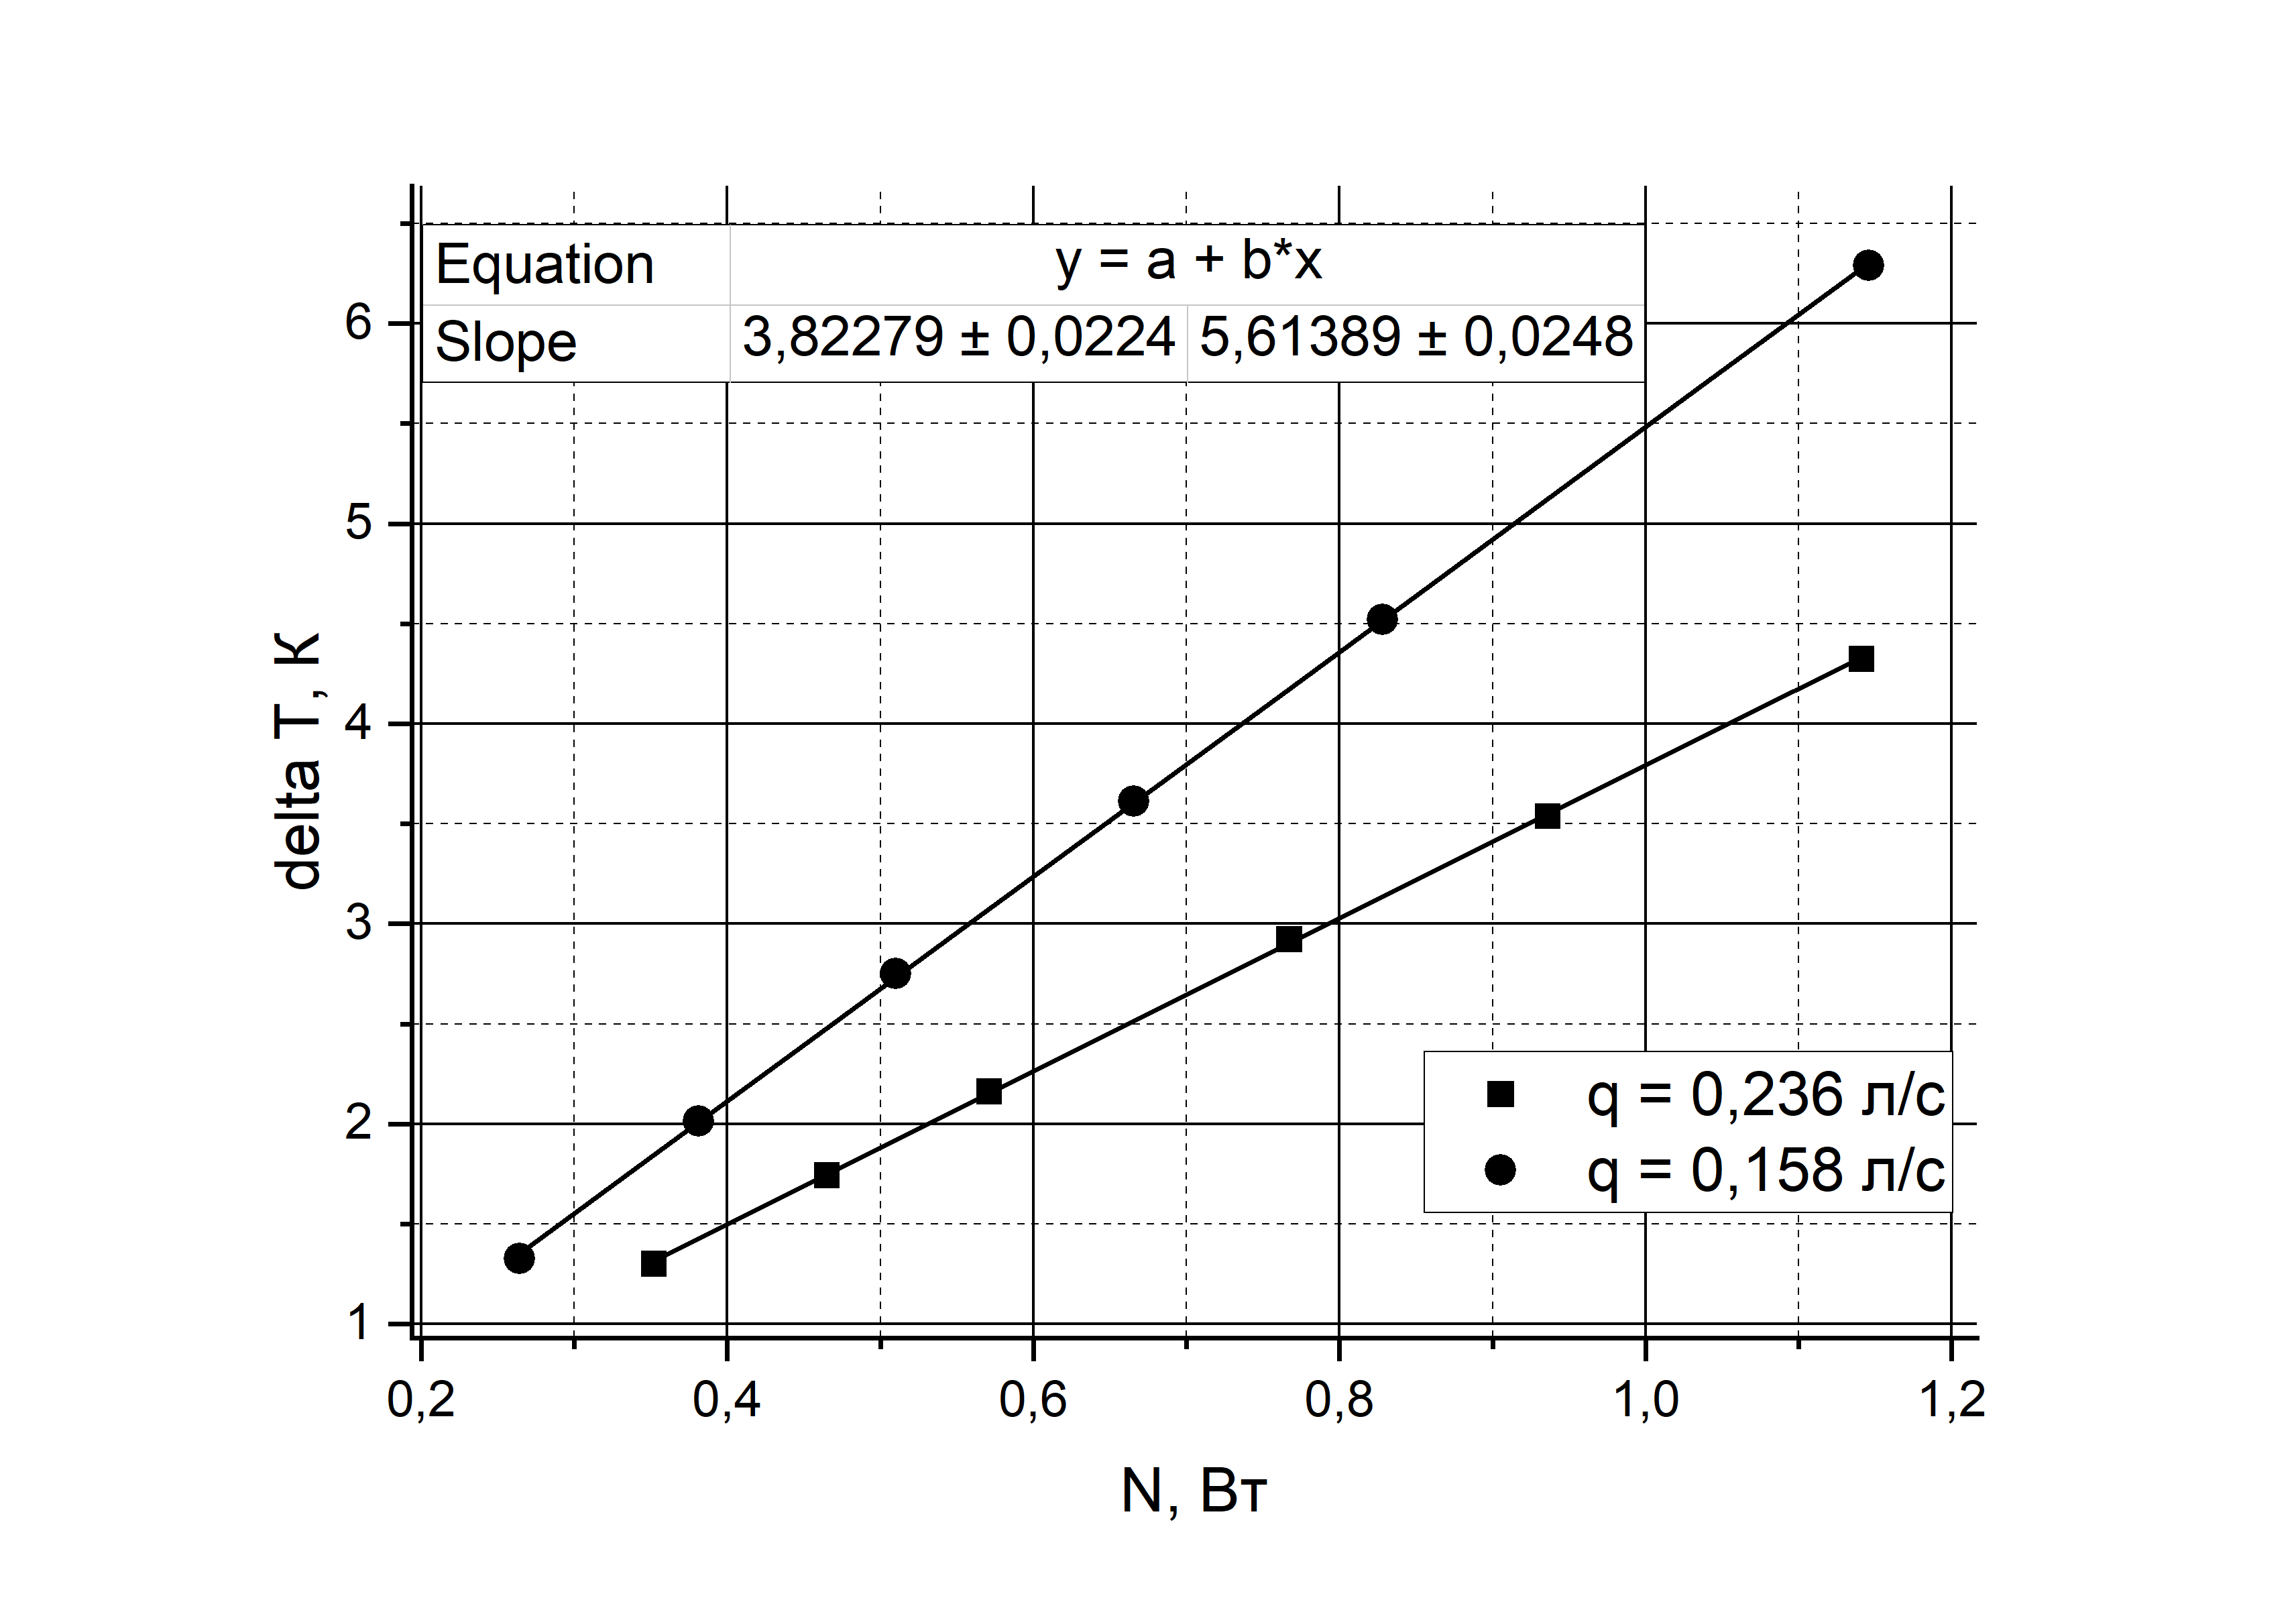
\includegraphics[width = 0.8\textwidth]{1.png}
	\end{center}
	\caption{Зависимость $\Delta T$ от N}
\end{figure}

\newpage


\begin{figure}[h!]
	\begin{center}
		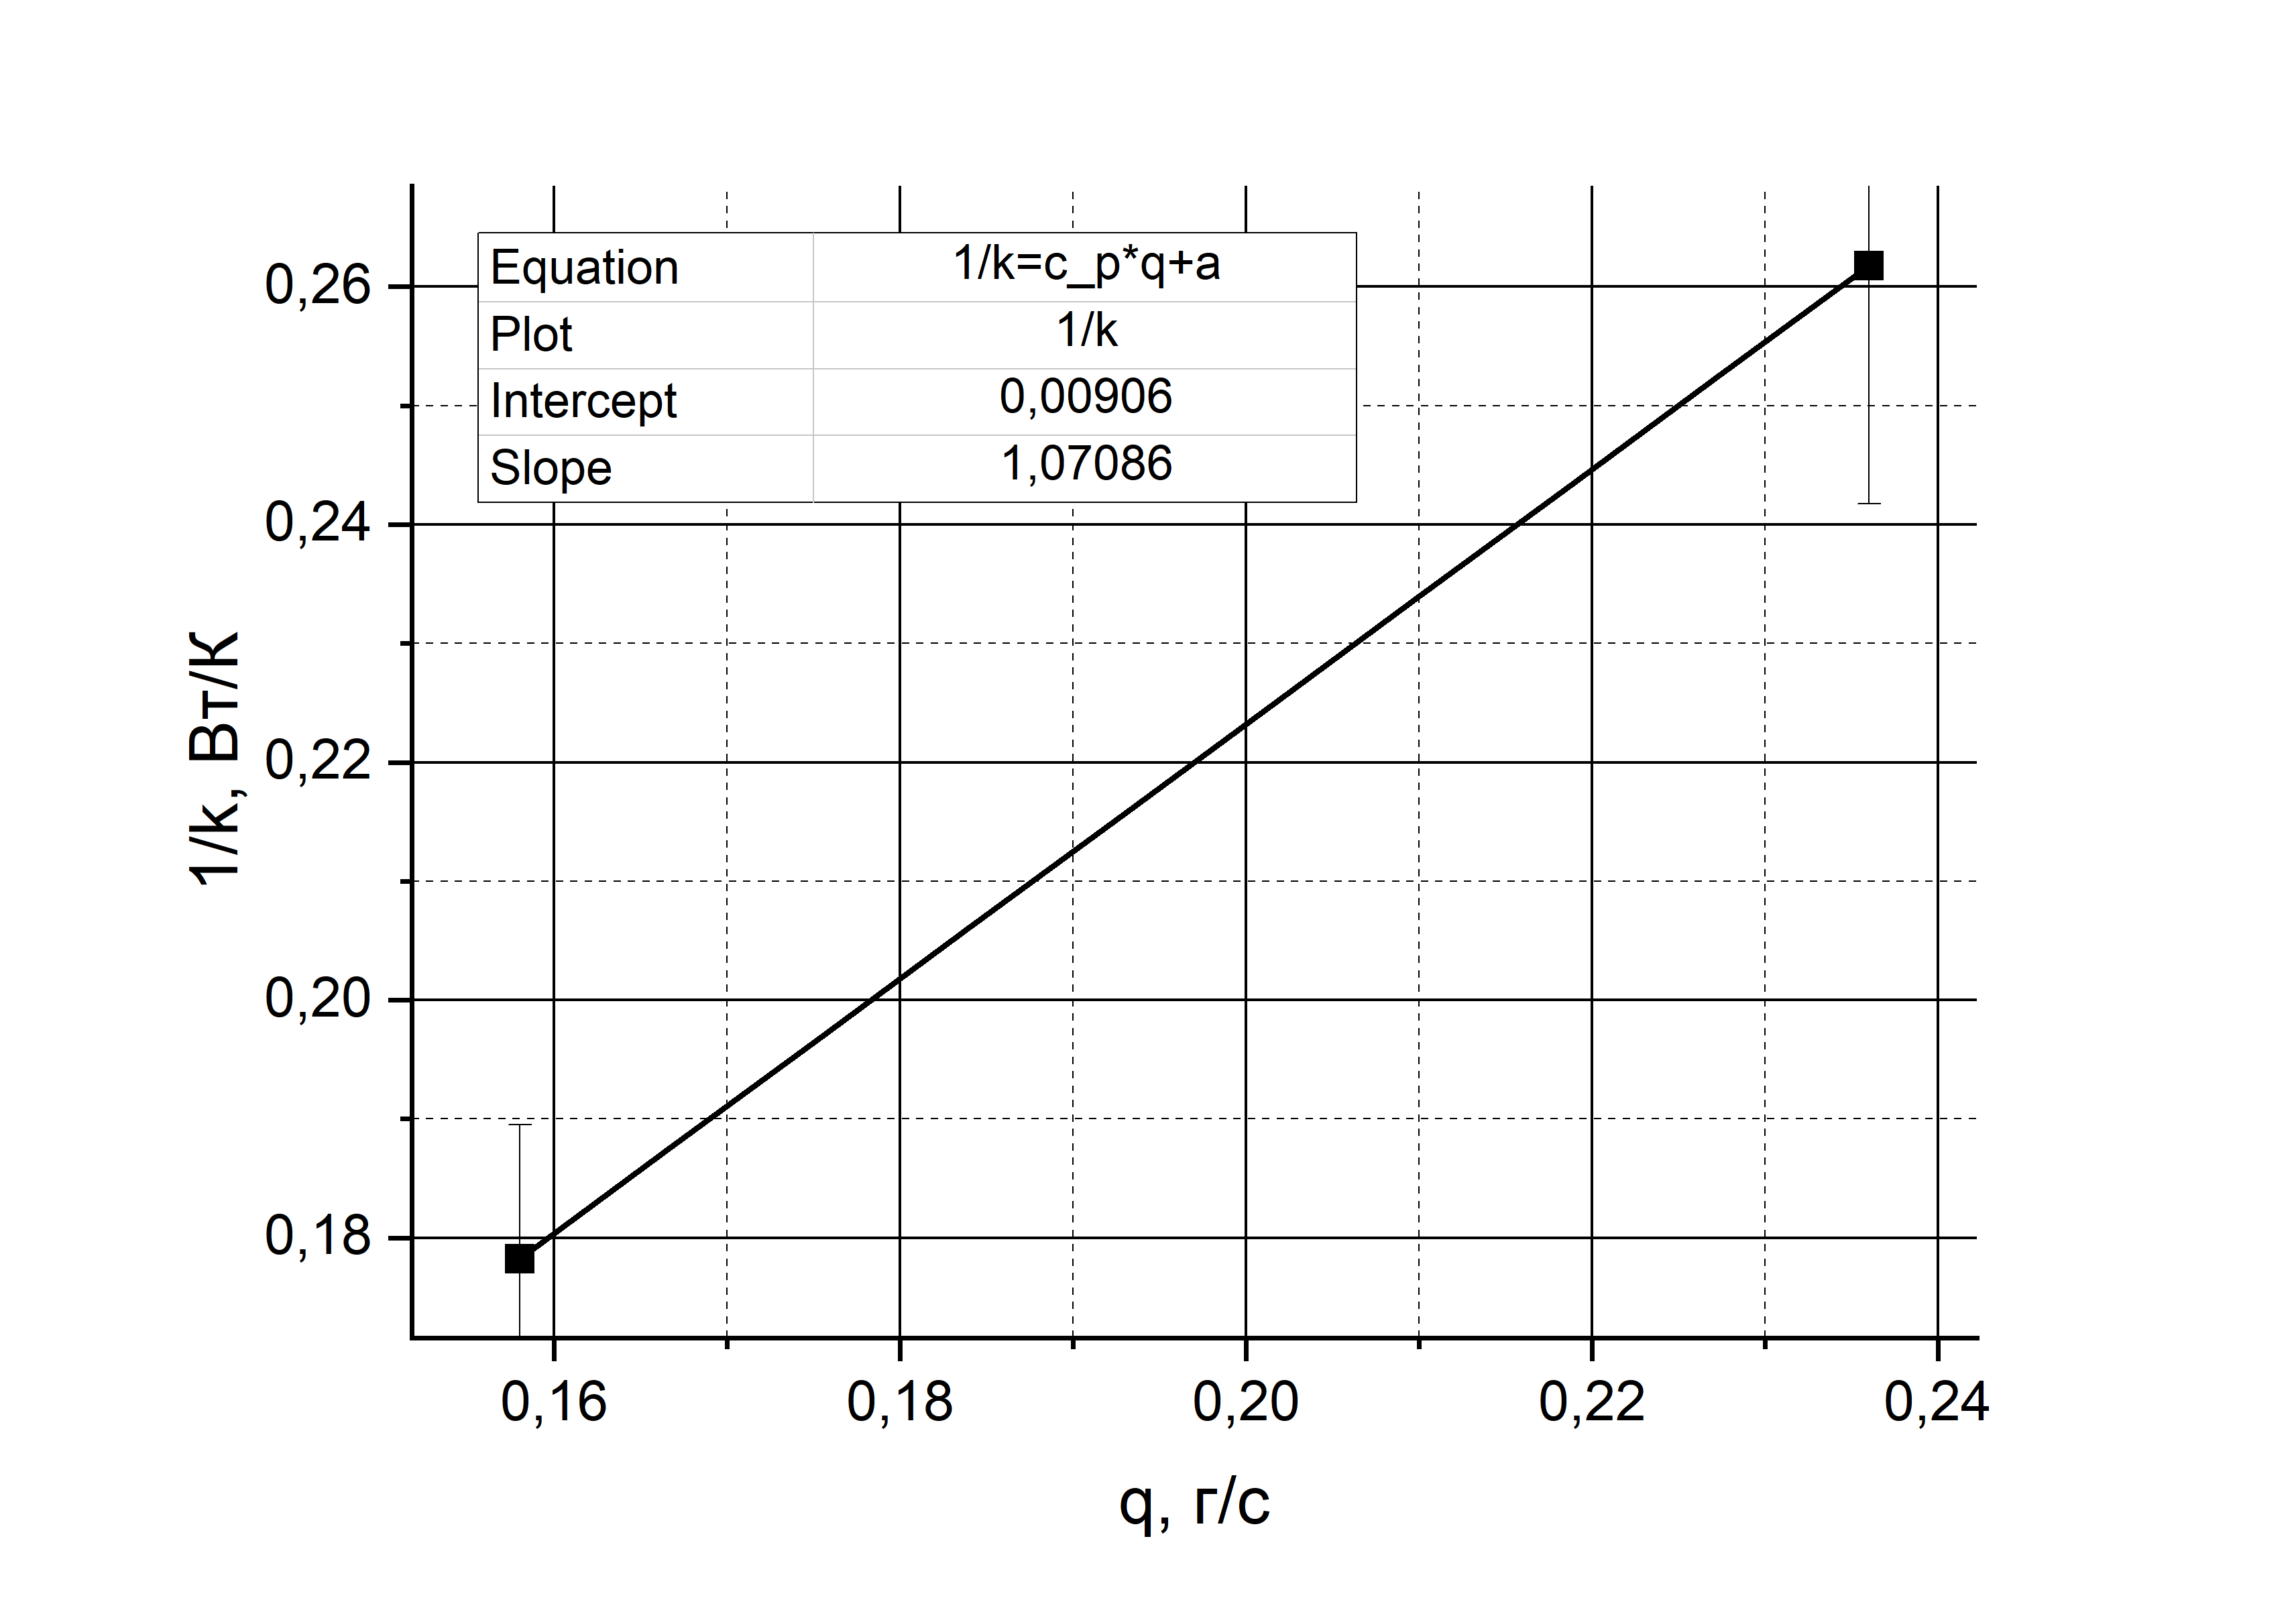
\includegraphics[width = 0.8\textwidth]{2.png}
	\end{center}
	\caption{Зависимость $\frac{1}{k}$ от q}
\end{figure}

\end{document}